% ==============================================================================
% Modelo para Projeto de Pesquisa de Doutorado (para processo seletivo)
% Programa de Pós-Graduação em Informática, Universidade Federal do Espírito Santo
%
% Baseado em abtex2-modelo-trabalho-academico.tex, v-1.9.2 laurocesar
% Copyright 2012-2014 by abnTeX2 group at http://abntex2.googlecode.com/ 
%
% Modificado por prof. Vítor E. Silva Souza
% http://www.inf.ufes.br/~vitorsouza/
%
% This work may be distributed and/or modified under the conditions of the LaTeX 
% Project Public License, either version 1.3 of this license or (at your option) 
% any later version. The latest version of this license is in
% http://www.latex-project.org/lppl.txt.
%
% IMPORTANTE:
% Instruções encontram-se espalhadas pelo documento. Para facilitar sua leitura,
% tais instruções são precedidas por (*) -- utilize a função localizar do seu
% editor para passar por todas elas.
% ==============================================================================

% Usa o estilo abntex2, configurando detalhes de formatação e hifenização.
\documentclass[
	article,           % Seções ao invés de capítulos.
	12pt,              % Tamanho da fonte.
	oneside,         % Para impressão em apenas um lado (não inclui páginas em branco).
	a4paper,        % Tamanho do papel.
	english,         % Idioma adicional para hifenização.
	french,	          % Idioma adicional para hifenização.
	spanish,        % Idioma adicional para hifenização.
	brazil             % O último idioma é o principal do documento.
	]{abntex2}



%%% Importação de pacotes. %%%

% Conserta o erro "No room for a new \count"
% Em alguns sistemas operacionais, a linha \reserveinserts{28} deve ser comentada.
\usepackage{etex}
%\reserveinserts{28}

% Usa a fonte Latin Modern.
\usepackage{lmodern}

% Seleção de códigos de fonte.
\usepackage[T1]{fontenc}

% Codificação do documento em Unicode.
\usepackage[utf8]{inputenc}

% Indenta o primeiro parágrafo de cada seção.
\usepackage{indentfirst}

% Controle das cores.
\usepackage[usenames,dvipsnames,table]{xcolor}

% Inclusão de gráficos.
\usepackage{graphicx}

% Para melhor personalização das tabelas.
\usepackage{tabularx}
\usepackage{multirow}
\usepackage{hhline}

% Para melhorias de justificação.
\usepackage{microtype}

% Citações padrão ABNT.
\usepackage[brazilian,hyperpageref]{backref}
\usepackage[alf]{abntex2cite}	
\renewcommand{\backrefpagesname}{Citado na(s) página(s):~}    % Usado sem a opção hyperpageref de backref.
\renewcommand{\backref}{}                                                              % Texto padrão antes do número das páginas.
\renewcommand*{\backrefalt}[4]{                                                     % Define os textos da citação.
	\ifcase #1
		Nenhuma citação no texto.
	\or
		Citado na página #2.
	\else
		Citado #1 vezes nas páginas #2.
	\fi}

% \rm is deprecated and should not be used in a LaTeX2e document
% http://tex.stackexchange.com/questions/151897/always-textrm-never-rm-a-counterexample
\renewcommand{\rm}{\textrm}

% Inclusão de símbolos não padrão.
\usepackage{amssymb}
\usepackage{eurosym}

% Para utilizar \eqref para referenciar equações.
\usepackage{amsmath}

% Permite mostrar figuras muito largas em modo paisagem com \begin{sidewaysfigure} ao invés de \begin{figure}.
\usepackage{rotating}

% Permite customizar listas enumeradas/com marcadores.
\usepackage{enumitem}

% Permite inserir hiperlinks com \url{}.
\usepackage{bigfoot}
\usepackage{hyperref}

% Permite usar o comando \hl{} para evidenciar texto com fundo amarelo. Útil para chamar atenção a itens a fazer.
\usepackage{soulutf8}

% Permite inserir comentários para viabilizar escrita colaborativa ou revisão pelo professor orientador.
\usepackage[colorinlistoftodos, textwidth=20mm, textsize=footnotesize]{todonotes}
\newcommand{\aluno}[1]{\todo[author=\textbf{Aluno},color=green!30,caption={},inline]{#1}}
\newcommand{\professor}[1]{\todo[author=\textbf{Professor},color=red!30,caption={},inline]{#1}}
\newcommand{\instrucoes}[1]{\todo[author=\textbf{Instruções para elaboração},color=blue!30,caption={},inline]{#1}}

% Permite inserir espaço em branco condicional (incluído no texto final só se necessário) em macros.
\usepackage{xspace}

% Permite incluir listagens de código com o comando \lstinputlisting{}.
\usepackage{listings}
\usepackage{caption}
\DeclareCaptionFont{white}{\color{white}}
\DeclareCaptionFormat{listing}{\colorbox{gray}{\parbox{\textwidth}{#1#2#3}}}
\captionsetup[lstlisting]{format=listing,labelfont=white,textfont=white}
\renewcommand{\lstlistingname}{Listagem}
\definecolor{mygray}{rgb}{0.5,0.5,0.5}
\lstset{
	basicstyle=\scriptsize,
	breaklines=true,
	numbers=left,
	numbersep=5pt,
	numberstyle=\tiny\color{mygray}, 
	rulecolor=\color{black},
	showstringspaces=false,
	tabsize=2,
    inputencoding=utf8,
    extendedchars=true,
    literate=%
    {é}{{\'{e}}}1
    {è}{{\`{e}}}1
    {ê}{{\^{e}}}1
    {ë}{{\¨{e}}}1
    {É}{{\'{E}}}1
    {Ê}{{\^{E}}}1
    {û}{{\^{u}}}1
    {ù}{{\`{u}}}1
    {â}{{\^{a}}}1
    {à}{{\`{a}}}1
    {á}{{\'{a}}}1
    {ã}{{\~{a}}}1
    {Á}{{\'{A}}}1
    {Â}{{\^{A}}}1
    {Ã}{{\~{A}}}1
    {ç}{{\c{c}}}1
    {Ç}{{\c{C}}}1
    {õ}{{\~{o}}}1
    {ó}{{\'{o}}}1
    {ô}{{\^{o}}}1
    {Õ}{{\~{O}}}1
    {Ó}{{\'{O}}}1
    {Ô}{{\^{O}}}1
    {î}{{\^{i}}}1
    {Î}{{\^{I}}}1
    {í}{{\'{i}}}1
    {Í}{{\~{Í}}}1
}



%%% Definição de variáveis. %%%

% (*) Substituir os <<textos>> abaixo com as informações apropriadas.
\titulo{<<Título>>}
\autor{<<Nome do Candidato>>}
\local{Vitória, ES}
\data{<<mês/ano>>}
\orientador{<<Nome do candidato a orientador no PPGI>>}
\instituicao{
  Universidade Federal do Espírito Santo -- UFES
  \par
  Centro Tecnológico
  \par
  Programa de Pós-Graduação em Informática}
\tipotrabalho{Proposta de Projeto de Pesquisa}

% Preâmbulo (tipo do trabalho, objetivo, nome da instituição, área de concentração, etc.).
\preambulo{Proposta de Projeto de Pesquisa apresentada como requisito para participação no processo de seleção para o curso de Doutorado em Ciência da Computação do Programa de Pós-Graduação em Informática da Universidade Federal do Espírito Santo.}

% Macros específicas do trabalho.
% (*) Inclua aqui termos que são utilizados muitas vezes e que demandam formatação especial.
% O exemplo abaixo inclue Java com TM em superscript.
% Use sempre \xspace para que o LaTeX inclua espaço em branco após a macro somente quando necessário.
\newcommand{\java}{Java\texttrademark\xspace}




%%% Configurações finais de aparência. %%%

% Altera o aspecto da cor azul.
\definecolor{blue}{RGB}{41,5,195}

% Informações do PDF.
\makeatletter
\hypersetup{
	pdftitle={\@title}, 
	pdfauthor={\@author},
	pdfsubject={\imprimirpreambulo},
	pdfcreator={LaTeX with abnTeX2},
	pdfkeywords={abnt}{latex}{abntex}{abntex2}{trabalho acadêmico}, 
	colorlinks=true,           % Colore os links (ao invés de usar caixas).
	linkcolor=blue,            % Cor dos links.
	citecolor=blue,            % Cor dos links na bibliografia.
	filecolor=magenta,      % Cor dos links de arquivo.
	urlcolor=blue,             % Cor das URLs.
	bookmarksdepth=4
}
\makeatother

% Espaçamentos entre linhas e parágrafos.
\setlength{\parindent}{1.3cm}
\setlength{\parskip}{0.2cm}



%%% Páginas iniciais do documento: capa, folha de rosto, ficha, resumo, tabelas, etc. %%%

% Compila o índice. <--- Desnecessário em Plano de Estudo.
%\makeindex

% Inicia o documento.
\begin{document}

% Retira espaço extra obsoleto entre as frases.
\frenchspacing


% Capa do trabalho (com brasão da UFES).
\begin{figure}[h]
	\centering
	
\includegraphics[scale=0.055]{figuras/brasao.jpg}
\end{figure} 
\imprimircapa

% Folha de rosto (o * indica que haverá a ficha bibliográfica). <--- Ficha bibliográfica desnecessária em Plano de Estudo.
\imprimirfolhaderosto

% Resumo.
% (*) Escrever resumo e palavras-chave.
\setlength{\absparsep}{18pt}
\begin{resumo}
	<<Resumo do projeto>>
	
	\textbf{Palavras-chaves}: <<lista de palavras-chave>>
	
	\instrucoes{\begin{itemize}
			\item O resumo deve ter entre 100 e 300 palavras;
			\item Devem ser informadas de 3 a 6 palavras-chave.
	\end{itemize}}
\end{resumo}


%%% Início da parte de conteúdo do documento. %%%

% Marca o início dos elementos textuais.
\clearpage
\textual

% Inclusão das seções.
% (*) Para facilitar a organização, as seções foram divididas em arquivo separados e colocadas dentro da
% pasta secoes. Caso o candidato prefira trabalhar com um só arquivo, basta substituir os comandos \include 
% pelos conteúdos dos arquivos que estão sendo incluídos, excluindo a pasta secoes/ em seguida.
% ==============================================================================
% Proposta de Projeto de Pesquisa - Nome do Aluno
% Seção 1 - Introdução
% ==============================================================================
\section{Introdução}
\label{sec-intro}

\instrucoes{\begin{itemize}
		\item No arquivo \texttt{.tex} principal, procure por \texttt{(*)} e insira seus dados para a capa do documento;
		\item Leia com atenção todas as instruções;
		\item Caso não tenha muita experiência com \LaTeX, leia o Apêndice~\ref{sec-dicaslatex};
		\item Antes de entregar a versão final do documento, exclua todas as instruções e o Apêndice~\ref{sec-dicaslatex};
		\item Use BibTeX para referências bibliográficas e não altere a formatação do modelo básico abnTeX2.\footnote{\url{http://www.abntex.net.br}.}
\end{itemize}

\textbf{Especificamente com relação a esta seção:}
\begin{itemize}
	\item A introdução deve: (i) introduzir o tema do projeto, justificando a sua atualidade e relevância; (ii) contextualizar a pesquisa e (iii) colocar o problema de pesquisa;
	\item As colocações/afirmativas devem ser respaldadas na literatura e/ou em experimentos;
	\item Deve ser capaz de mostrar a importância e relevância da pesquisa proposta;
	\item Número de páginas: entre 1 e 3 páginas.
\end{itemize}}

% ==============================================================================
% Proposta de Projeto de Pesquisa - Nome do Aluno
% Seção 2 - Referencial Teórico
% ==============================================================================
\section{Referencial Teórico}
\label{sec-refer}

\instrucoes{\begin{itemize}
		\item Nesta seção devem ser abordados os conceitos extraídos da literatura sobre o tema ou especificamente sobre o problema;
		\item Este deve ser o tópico mais desenvolvido neste projeto;
		\item Pode ser organizado em subseções, cada uma abordando um tópico relacionado ao trabalho de pesquisa;
		\item Número de páginas: entre 3 e 5 páginas.
	\end{itemize}}

% ==============================================================================
% Proposta de Projeto de Pesquisa - Nome do Aluno
% Seção 3 - Objetivos
% ==============================================================================
\section{Objetivos}
\label{sec-objeto}

Este trabalho tem como objetivo geral <<objetivo geral>>. Esse objetivo geral pode ser detalhado nos seguintes objetivos específicos:

\begin{itemize}
	\item <<objetivo específico 1>>;
	\item <<objetivo específico 2>>;
	\item <<etc...>>.
\end{itemize}

\instrucoes{\begin{itemize}
		\item Deve apresentar claramente o objetivo geral e os objetivos específicos da pesquisa e somente isso;
		\item Os objetivos devem ser expressos por meio de verbos no infinitivo;
		\item Observar que objetivos específicos não devem ser confundidos com atividades do método de pesquisa, o qual deve ser apresentado na Seção~\ref{sec-metodo}.
	\end{itemize}}

% ==============================================================================
% Proposta de Projeto de Pesquisa - Nome do Aluno
% Seção 4 - Justificativas
% ==============================================================================
\section{Justificativas}
\label{sec-justif}

\instrucoes{\begin{itemize}
		\item Esta seção deve apresentar justificativas para o projeto e, quando pertinente, hipóteses consideradas e limitações do trabalho;
		\item Idealmente, uma boa justificativa para uma hipótese apresenta uma limitação a abordagens existentes e justifica, com base nisso, uma potencial solução, explicando por que ela seria adequada;
		\item Número de páginas: entre 1 e 2 páginas.
\end{itemize}}

% ==============================================================================
% Plano de Estudo no Exterior - Nome do Aluno
% Seção 5 - Método de Pesquisa
% ==============================================================================
\section{Método de Pesquisa}
\label{sec-metodo}

<<Descrição do método de pesquisa a ser adotado, seguido das atividades previstas>>

Para atingir os objetivos listados na Seção~\ref{sec-objeto}, as seguintes atividades serão realizadas:

\begin{enumerate}
	\item <<Atividade 1>>;
	\item <<Atividade 2>>;
	\item <<etc...>>.
\end{enumerate}

\instrucoes{\begin{itemize}
		\item Deve indicar como o trabalho de pesquisa será conduzido;
		\item Deve ser concluído com a enumeração das atividades a serem realizadas, conforme acima;
		\item Número máximo de páginas: entre 1 e 3 páginas.
\end{itemize}}

% ==============================================================================
% Plano de Estudo no Exterior - Nome do Aluno
% Seção 6 - Cronograma
% ==============================================================================
\section{Cronograma}
\label{sec-crono}

\begin{center}
\footnotesize 
\begin{tabular}{ | c | c | c | c | c | c | c | c | c | c | c | c | c | c | c | c | c |}\hline
	\rowcolor{gray!30} & \multicolumn{16}{|c|}{\textbf{Trimestre}}\\\hhline{~|----------------}
	\rowcolor{gray!30}\textbf{Atividade} &  \multicolumn{4}{|c|}{\textbf{<<Ano1>>}} & \multicolumn{4}{|c|}{\textbf{<<Ano2>>}} & \multicolumn{4}{|c|}{\textbf{<<Ano3>>}} & \multicolumn{4}{|c|}{\textbf{<<Ano4>>}}\\\hhline{~|----------------}
	\rowcolor{gray!30} & \textbf{01} & \textbf{02} & \textbf{03} & \textbf{04} & \textbf{05} & \textbf{06} & \textbf{07} & \textbf{08} & \textbf{09} & \textbf{10} & \textbf{11} & \textbf{12} & \textbf{13} & \textbf{14} & \textbf{15} & \textbf{16}\\\hline
	\cellcolor{gray!30}\textbf{1} & & & & & & & & & & & & & & & & \\\hline
	\cellcolor{gray!30}\textbf{2} & & & & & & & & & & & & & & & & \\\hline
	\cellcolor{gray!30}\textbf{3} & & & & & & & & & & & & & & & & \\\hline
	\cellcolor{gray!30}\textbf{4} & & & & & & & & & & & & & & & & \\\hline
	\cellcolor{gray!30}\textbf{5} & & & & & & & & & & & & & & & & \\\hline
	\cellcolor{gray!30}\textbf{6} & & & & & & & & & & & & & & & & \\\hline
\end{tabular}
\end{center}

\instrucoes{\begin{itemize}
		\item O cronograma deve ser organizado em trimestres e deve contemplar os quatro anos de duração do curso,\footnote{Segundo o Regimento Interno do PPGI, o prazo máximo para concluir o doutorado é de 60 meses. No entanto, orienta-se que o cronograma do projeto de doutorado seja elaborado considerando-se 48 meses, que é o tempo considerado ideal para a conclusão do doutorado. Ao longo do trabalho, caso haja necessidade de estender o tempo de desenvolvimento, o aluno poderá utilizar o tempo ainda disponível até o prazo máximo permitido.} conforme tabela acima;
		\item Substitua <<Ano1>>, <<Ano2>>, <<Ano3>> e <<Ano4>> pelos anos correspondentes;
		\item Os números das atividades na primeira coluna devem corresponder às atividades descritas na Seção~\ref{sec-metodo} (Metodologia). Adicione/remova linhas se necessário, marque com um X os meses em que as atividades serão realizadas.
\end{itemize}}





%%% Páginas finais do documento: bibliografia e anexos. %%%

% Finaliza a parte no bookmark do PDF para que se inicie o bookmark na raiz e adiciona espaço de parte no sumário.
\phantompart

% Marca o início dos elementos pós-textuais.
\postextual

% Referências bibliográficas
\bibliography{bibliografia}


% Apêndices.
% (*) Incluído apenas para dar dicas de LaTeX. Remover/comentar antes de entregar o plano de estudo.
\begin{apendicesenv}
\partapendices
% ==============================================================================
% Dicas de Uso do LaTeX
% ==============================================================================
\section{Dicas de uso do \LaTeX}
\label{sec-dicaslatex}

Além do template pronto para uso, este documento inclui exemplos de uso de \LaTeX\ que podem ser úteis para aqueles que possuem pouca experiência com a ferramenta. Quando for começar a escrever seu documento, apague este apêndice.



%%% Início de seção. %%%
\subsection{Seções e subseções}
\label{sec-dicaslatex-secoes}

Documentos podem ser organizados em capítulos (\texttt{\textbackslash chapter\{\}}), seções (\texttt{\textbackslash section\{\}}), subseções (\texttt{\textbackslash subsection\{\}}), sub-subseções (\texttt{\textbackslash subsubsection\{\}}) e assim por diante. Atenção, porém, a não criar estruturas muito profundas (sub-sub-sub-...) pois o documento não fica bem estruturado.


%%% Início de seção. %%%
\subsubsection{Referências a seções}
\label{sec-dicaslatex-secoes-refs}

Cada parte do documento (capítulo, seção, etc.) deve possuir um rótulo logo abaixo de sua definição. Por exemplo, esta seção é definida com \texttt{\textbackslash subsection\{Referências a seções\}} seguido por \texttt{\textbackslash label\{sec-dicaslatex-secoes-refs\}}. Assim, podemos fazer referências cruzadas usando o comando \texttt{\textbackslash ref\{rótulo\}}: ``A Seção~\ref{sec-dicaslatex} começa com a Subseção~\ref{sec-dicaslatex-secoes}, que é ainda subdividida nas subseções~\ref{sec-dicaslatex-secoes-refs} e~\ref{sec-dicaslatex-secoes-sobrerefs}.

Para melhor organização das partes do documento, sugere-se primeiro utilizar o prefixo \texttt{sec-} (para diferenciar de referências à figuras, tabelas, etc. quando usarmos o comando \texttt{\textbackslash ref\{\}}) e também representar a hierarquia das seções nos rótulos. Por exemplo, a Seção~\ref{sec-dicaslatex} tem rótulo \texttt{sec-dicaslatex}, sua Subseção~\ref{sec-dicaslatex-secoes} tem rótulo \texttt{sec-dicaslatex-secoes} e a Subsubseção~\ref{sec-dicaslatex-secoes-refs} tem rótulo \texttt{sec-dicaslatex-secoes-refs}.



%%% Início de seção. %%%
\subsubsection{Sobre referências cruzadas}
\label{sec-dicaslatex-secoes-sobrerefs}

Nas próximas seções, veremos que é possível fazer referência cruzada não só a seções mas também a listagens de código, figuras, tabelas, etc. Em todos estes casos, quando nos referimos à Seção X, Listagem Y ou Figura Z, consideramos que estes são os nomes próprios destes elementos e, portanto, usa-se a primeira letra maiúscula. Isso pode ser visto na Subseção~\ref{sec-dicaslatex-secoes-refs}, acima. A exceção é quando nos referimos a vários elementos ao mesmo tempo, por exemplo: ``as subseções~\ref{sec-dicaslatex-secoes-refs} e~\ref{sec-dicaslatex-secoes-sobrerefs}''.

Por fim, ao usar o comando \texttt{\textbackslash ref\{\}}, sugere-se separá-lo da palavra que vem antes dele com um \textasciitilde\ ao invés de espaço. Por exemplo: \texttt{a Seção\textasciitilde \textbackslash ref\{sec-dicaslatex\}}. Isso faz com que o \LaTeX\ não quebre linha entre a palavra \texttt{Seção} e o número da seção. Note que ao usar a palavra \emph{seção} junto com seu número, ela deve ser usada com a inicial maiúscula por se tratar de um nome próprio: Seção~\ref{sec-dicaslatex}. O mesmo vale para figuras, tabelas, etc.




%%% Início de seção. %%%
\subsection{Citações bibliográficas}
\label{sec-dicaslatex-citacoes}

Este documento utiliza a ferramenta de gerenciamento de referências bibliográficas do \LaTeX, chamada \emph{BibTeX}. O arquivo \texttt{bibliografia.bib}, referenciado no arquivo \LaTeX\ principal deste documento, contém algumas referências bibliográficas de exemplo. Assim como capítulos, seções, etc., tais referências também possuem rótulos, especificados como primeiro parâmetro de cada entrada (ex.: \texttt{@incollection\{souza-et-al:iism08, ...\}}.

Sugere-se um padrão para rótulos de referências bibliográficas para que fique claro também no código \LaTeX\ qual referência está sendo citada. Por exemplo, ao citar a referência \texttt{souza-et-al:sesas13}, sabemos que é um artigo escrito por \emph{Souza} e outros, publicado no \emph{SESAS} em \emph{2013} (geralmente a pessoa que citou sabe que publicação é SESAS e quem é Souza).

Para citar uma referência bibliográfica contida no arquivo \emph{BibTeX}, basta usar seu rótulo como parâmetro de um de dois comandos possíveis de citação:

\begin{itemize}
\item O comando \texttt{\textbackslash cite\{\}} efetua uma citação tradicional, colocando o nome do(s) autor(es) e o ano entre parênteses. Por exemplo, \texttt{\textbackslash cite\{souza-et-al:iism08\}} é transformado em \cite{souza-et-al:iism08};

\item O comando \texttt{\textbackslash citeonline\{\}} efetua uma citação integrada ao texto, colocando o nome do(s) autor(es) direto no texto e somente o ano entre parênteses. Por exemplo, ``de acordo com \texttt{\textbackslash citeonline\{souza-et-al:iism08\}}'' é transformado em: de acordo com \citeonline{souza-et-al:iism08};
\end{itemize}

Também é possível citar vários trabalhos de uma só vez, separando os rótulos das referências bibliográficas com uma vírgula dentro do comando apropriado. Por exemplo, \texttt{\textbackslash cite\{souza-et-al:sesas13,souza-et-al:csrd13\}} \cite{souza-et-al:sesas13,souza-et-al:csrd13}.

Os trabalhos citados são automaticamente incluídos na seção de referências bibliográficas, ao final do documento. Tudo é formatado automaticamente segundo padrões da ABNT.



%%% Início de seção. %%%
\subsection{Listagens de código}
\label{sec-dicaslatex-listagens}

O pacote \texttt{listings}, incluído neste template, permite a inclusão de listagens de código. Análogo ao já feito anteriormente, listagens possuem rótulos para que possam ser referenciadas e sugerimos uma regra de nomenclatura para tais rótulos: usar como prefixo o rótulo do capítulo, substituindo \texttt{sec-} por \texttt{lst-}.

A Listagem~\ref{lst-dicaslatex-exemplo}, por exemplo, possui o rótulo \texttt{lst-dicaslatex-exemplo} e representa o código que foi usado no próprio documento para exibir as listagens desta seção. Como podemos ver, a sugestão é que os arquivos de código sejam colocados dentro da pasta \texttt{codigos/} e tenham nome idêntico ao rótulo, colocando a extensão adequada ao tipo de código.

\lstinputlisting[label=lst-dicaslatex-exemplo, caption=Exemplo de código \LaTeX\ para inclusão de listagens de código., float=htpb]{codigos/lst-dicaslatex-exemplo.tex}

A Listagem~\ref{lst-dicaslatex-outroexemplo} mostra um exemplo de listagem com especificação da linguagem utilizada no código. O pacote \texttt{listings} reconhece algumas linguagens\footnote{Veja a lista de linguagens suportadas em \url{http://en.wikibooks.org/wiki/LaTeX/Source\_Code\_Listings\#Supported_languages}.} e faz ``coloração'' de código (na verdade, usa \textbf{negrito} e não cores) de acordo com a linguagem. O parâmetro \texttt{float=htpb} incluído em ambos os exemplos impede que a listagem seja quebrada em diferentes páginas.

\lstinputlisting[label=lst-dicaslatex-outroexemplo, caption=Exemplo de código \java especificando linguagem utilizada., language=Java, float=htpb]{codigos/lst-dicaslatex-outroexemplo.java}



%%% Início de seção. %%%
\subsection{Figuras}
\label{sec-dicaslatex-figuras}

Figuras podem ser inseridas no documento usando o \emph{ambiente} \texttt{figure} (ou seja, \texttt{\textbackslash begin\{figure\}} e \texttt{\textbackslash end\{figure\}}) e o comando \texttt{\textbackslash includegraphics\{\}}. Existem alguns outros elementos e propriedades úteis de serem configuradas, resultando no código exibido na Listagem~\ref{lst-dicaslatex-figuras}.

\lstinputlisting[label=lst-dicaslatex-figuras, caption=Código \LaTeX\ utilizado para inclusão das figuras na Seção~\ref{sec-dicaslatex-figuras}., float=htpb]{codigos/lst-dicaslatex-figuras.tex}

O comando \texttt{\textbackslash centering} centraliza a figura na página. A opção \texttt{width} do comando \texttt{\textbackslash includegraphics\{\}} determina o tamanho da figura e usa-se \texttt{\textbackslash textwidth} (opcionalmente multiplicado por um número) para se referir à largura da página. O parâmetro do comando \texttt{\textbackslash includegraphics\{\}} indica onde a imagem pode ser encontrada. Foi criado o diretório \texttt{figuras/} para conter as figuras do documento, dando uma melhor organização aos arquivos.

Por fim, o comando \texttt{\textbackslash caption\{\}} especifica a descrição da figura e \texttt{\textbackslash label\{\}}, como de costume, estabelece um rótulo para permitir referência cruzada de figuras. Note ainda que é utilizada a mesma estratégia de nomenclatura de rótulos usada nas listagens, porém utilizando o prefixo \texttt{fig-}.

As figuras~\ref{fig-dicaslatex-nemologo} e~\ref{fig-dicaslatex-exemplosideways} mostram o resultado do código da Listagem~\ref{lst-dicaslatex-figuras}. A Figura~\ref{fig-dicaslatex-exemplosideways}, em particular, utiliza o pacote \texttt{rotating} para mostrar figuras largas em modo paisagem. Basta usar o ambiente \texttt{sidewaysfigure} ao invés de \texttt{figure}. Já a Figura~\ref{fig-dicaslatex-nemologo} utiliza o parâmetro \texttt{[h!]} que indica para o \LaTeX\ que a figura deve ser colocada na posição em que está em relação aos parágrafos (a regra geral é incluir a figura abaixo do primeiro parágrafo que a cita), se houver espaço. Sem este parâmetro o \LaTeX\ pode decidir colocar as figuras sempre no topo da página. Questão de gosto/estilo.

\begin{figure}[h!]
	\centering
	
\includegraphics[width=.25\textwidth]{figuras/fig-dicaslatex-nemologo} 
	\caption{Exemplo de figura: logo do NEMO.}
	\label{fig-dicaslatex-nemologo}
\end{figure}

\begin{sidewaysfigure}
\centering
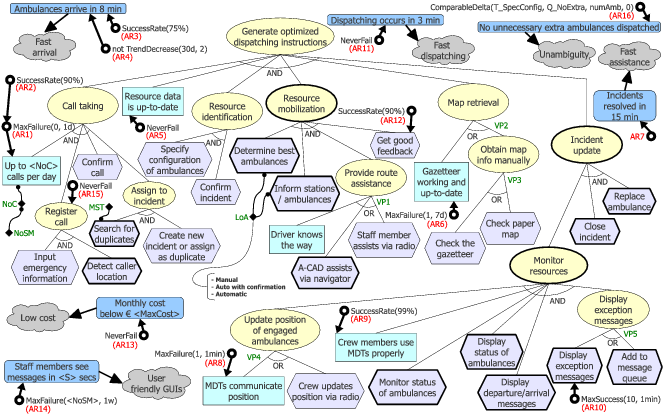
\includegraphics[width=\textwidth]{figuras/fig-dicaslatex-exemplosideways} 
\caption{Exemplo de figura em modo paisagem: um modelo de objetivos~\cite{souza-mylopoulos:spe13}.}
\label{fig-dicaslatex-exemplosideways}
\end{sidewaysfigure}



%%% Início de seção. %%%
\subsection{Tabelas}
\label{sec-dicaslatex-tabelas}

Tabelas são um ponto fraco do \LaTeX. Elas são complicadas de fazer e, dependendo da complexidade da tabela (muitas células mescladas, por exemplo), vale a pena construi-las em outro programa (por exemplo, em seu editor de texto favorito) e inclui-las no documento como figuras (ex.: tirando um screenshot da tela). Mostramos, no entanto, alguns exemplos de tabela a seguir. O código utilizado para criar as tabelas encontra-se nas listagens~\ref{lst-dicaslatex-tabelas01}, \ref{lst-dicaslatex-tabelas02} e~\ref{lst-dicaslatex-tabelas03}.

\lstinputlisting[label=lst-dicaslatex-tabelas01, caption=Código \LaTeX\ utilizado para inclusão das tabelas~\ref{tbl-dicaslatex-exemplo01} e~\ref{tbl-dicaslatex-exemplo02}., float=htpb]{codigos/lst-dicaslatex-tabelas01.tex}

\lstinputlisting[label=lst-dicaslatex-tabelas02, caption=Código \LaTeX\ utilizado para inclusão da Tabela~\ref{tbl-dicaslatex-exemplo03}., float=htpb]{codigos/lst-dicaslatex-tabelas02.tex}

\lstinputlisting[label=lst-dicaslatex-tabelas03, caption=Código \LaTeX\ utilizado para inclusão da Tabela~\ref{tbl-dicaslatex-exemplo04}., float=htpb]{codigos/lst-dicaslatex-tabelas03.tex}

Em particular, a Tabela~\ref{tbl-dicaslatex-exemplo04} utiliza um pacote chamado \texttt{tabularx}, que permite maior controle do layout das tabelas. Ao definir o ambiente \texttt{\textbackslash begin\{tabularx\}}, são definidos os tamanhos de cada coluna proporcional à largura ocupada pela tabela. Veja na Listagem~\ref{lst-dicaslatex-tabelas03} que as primeiras duas colunas não definem o atributo \texttt{\textbackslash hsize}, o que faz com que elas fiquem com o tamanho padrão de coluna, que é a largura da tabela dividida pelo número de colunas. Já a terceira coluna define \texttt{\textbackslash hsize=1.2\textbackslash hsize}, ou seja, esta coluna deve ser 20\% maior do que o tamanho padrão. Para isso, é preciso retirar de outras colunas, portanto a quarta e quinta colunas são definidas como 10\% menores (ou seja, \texttt{\textbackslash hsize=0.9\textbackslash hsize}).

% Exemplo de tabela 01:
\begin{table}
\caption{Exemplo de tabela com diferentes alinhamentos de conteúdo.}
\label{tbl-dicaslatex-exemplo01}
\centering
\begin{tabular}{ | c | l | r | p{40mm} |}\hline
\textbf{Centralizado} & \textbf{Esquerda} & \textbf{Direita} & \textbf{Parágrafo}\\\hline
C & L & R & Alinhamento de tipo parágrafo especifica largura da coluna e quebra o texto automaticamente.\\
\hline
Linha 2 & Linha 2 & Linha 2 & Linha 2\\
\hline
\end{tabular}
\end{table}

% Exemplo de tabela 02:
\begin{table}
\caption{Exemplo que especifica largura de coluna e usa lista enumerada (adaptada de~\cite{souza-mylopoulos:spe13}).}
\label{tbl-dicaslatex-exemplo02}
\centering
\renewcommand{\arraystretch}{1.2}
\begin{small}
\begin{tabular}{ | p{15mm} | p{77mm} | p{55mm} |}\hline
\textbf{\textit{AwReq}} & \textbf{Adaptation strategies} & \textbf{Applicability conditions}\\\hline

AR1 &
\vspace{-2mm}\begin{enumerate}[topsep=0cm, partopsep=0cm, itemsep=0cm, parsep=0cm, leftmargin=0.5cm]
\item \textit{Warning(``AS Management'')}
\item \textit{Reconfigure($\varnothing$)}
\end{enumerate}\vspace{-4mm} &
\vspace{-2mm}\begin{enumerate}[topsep=0cm, partopsep=0cm, itemsep=0cm, parsep=0cm, leftmargin=0.5cm]
\item Once per adaptation session;
\item Always.
\end{enumerate}\vspace{-4mm}
\\\hline

AR2 &
\vspace{-2mm}\begin{enumerate}[topsep=0cm, partopsep=0cm, itemsep=0cm, parsep=0cm, leftmargin=0.5cm]
\item \textit{Warning(``AS Management'')}
\item \textit{Reconfigure($\varnothing$)}
\end{enumerate}\vspace{-4mm} &
\vspace{-2mm}\begin{enumerate}[topsep=0cm, partopsep=0cm, itemsep=0cm, parsep=0cm, leftmargin=0.5cm]
\item Once per adaptation session;
\item Always.
\end{enumerate}\vspace{-4mm}
\\\hline
\end{tabular}
\end{small}
\end{table}

% Exemplo de tabela 03:
\begin{table}
\caption{Exemplo que mostra equações em duas colunas (adaptada de~\cite{souza-mylopoulos:spe13}).}
\label{tbl-dicaslatex-exemplo03}
\centering
\vspace{1mm}
\fbox{\begin{minipage}{.98\linewidth}
\begin{minipage}{0.51\linewidth}
\vspace{-4mm}
\begin{eqnarray}
\Delta \left( I_{AR1} / NoSM \right) \left[ 0, maxSM \right] > 0\\
\Delta \left( I_{AR2} / NoSM \right) \left[ 0, maxSM \right] > 0\\
\Delta \left( I_{AR3} / LoA \right) < 0\\
\end{eqnarray}
\vspace{-6mm}
\end{minipage}
\hspace{2mm}
\vline 
\begin{minipage}{0.41\linewidth}
\vspace{-4mm}
\begin{eqnarray}
\Delta \left( I_{AR11} / VP2 \right) < 0\\
\Delta \left( I_{AR12} / VP2 \right) > 0\\
\Delta \left( I_{AR6} / VP3 \right) > 0\\
\end{eqnarray}
\vspace{-6mm}
\end{minipage}
\end{minipage}}
\end{table}

% Exemplo de tabela 04:
\begin{table}[h]
	\caption{Exemplo que utiliza o pacote \texttt{tabularx}, extraído de um artigo não publicado.}
	\label{tbl-dicaslatex-exemplo04}
	\centering\tiny\def\tabularxcolumn#1{m{#1}}
	\begin{tabularx}{\columnwidth}{ >{\centering}X | >{\centering}X | >{\hsize=1.2\hsize\centering}X | >{\hsize=0.9\hsize\centering}X | >{\hsize=0.9\hsize\centering\arraybackslash}X }
		\hline
		\textbf{Applied Criteria} & \textbf{Analyzed Content} & \textbf{Initial\\Occurrences} & \textbf{Final Results} & \textbf{Reduction (\%)} \\
		\hline
		Duplicate Removal & Title, authors and year & 903 & 420 & 54,84\% \\ 
		\hline 
		IC and ECs & Title, abstract and keywords & 420 & 130 & 69,05\% \\ 
		\hline 
		IC and ECs & Full text & 130 & 117 & 10\% \\ 
		\hline 
		Final Results & -- & 903 & 117 & 87,04\% \\ 
		\hline 
	\end{tabularx}
\end{table}
\end{apendicesenv}


% Fim do documento.
\end{document}
